
%% Beginning of file 'sample63.tex'
%%
%% Modified 2019 June
%%
%% This is a sample manuscript marked up using the
%% AASTeX v6.3 LaTeX 2e macros.
%%
%% AASTeX is now based on Alexey Vikhlinin's emulateapj.cls 
%% (Copyright 2000-2015).  See the classfile for details.

%% AASTeX requires revtex4-1.cls (http://publish.aps.org/revtex4/) and
%% other external packages (latexsym, graphicx, amssymb, longtable, and epsf).
%% All of these external packages should already be present in the modern TeX 
%% distributions.  If not they can also be obtained at www.ctan.org.

%% The first piece of markup in an AASTeX v6.x document is the \documentclass
%% command. LaTeX will ignore any data that comes before this command. The 
%% documentclass can take an optional argument to modify the output style.
%% The command below calls the preprint style which will produce a tightly 
%% typeset, one-column, single-spaced document.  It is the default and thus
%% does not need to be explicitly stated.
%%
%%
%% using aastex version 6.3
\documentclass[twoside,twocolumn]{aastex63}
\usepackage{amsmath}
\usepackage[T1]{fontenc}
%\usepackage[margin=2cm]{geometry}  % only to bring all on one page
\usepackage{url}
\usepackage{graphicx}
\usepackage[caption=false]{subfig}
%\captionsetup{compatibility=false}
%
\DeclareCaptionFormat{cont}{#1 (continued.)#2#3\par}

\newcommand{\vdag}{(v)^\dagger}
\newcommand\aastex{AAS\TeX}
\newcommand\latex{La\TeX}

%% Reintroduced the \received and \accepted commands from AASTeX v5.2
%\received{June 1, 2019}
%\revised{January 10, 2019}
%\accepted{\today}
%% Command to document which AAS Journal the manuscript was submitted to.
%% Adds "Submitted to " the argument.
%\submitjournal{ApJ}
\shorttitle{Periodic X-ray Sources in the Galactic Bulge}
\shortauthors{Bao \& Li}
\begin{document}
\title{Periodic Cataclysmic Variables in the Galactic Bulge: Application of the Gregory-Loredo Algorithm}

%\correspondingauthor{August Muench}
%\email{greg.schwarz@aas.org, gus.muench@aas.org}

\author{Tong Bao}
\affiliation{School of Astronomy and Space Science, Nanjing University, Nanjing 210046, China}
\affiliation{Key Laboratory of Modern Astronomy and Astrophysics (Nanjing University), Ministry of Education, Nanjing 210046, China}
\author{Zhiyuan Li}
\affiliation{School of Astronomy and Space Science, Nanjing University, Nanjing 210046, China}
\affiliation{Key Laboratory of Modern Astronomy and Astrophysics (Nanjing University), Ministry of Education, Nanjing 210046, China}
\begin{abstract}
We present the discovery of 22 X-ray periodic sources in the Limiting Window (LW), a low-extinction region in the Galactic bulge, locating 80' south of the Galactic center. Their luminosities range(${\rm 10^{31}-10^{33} ~erg ~ s^{-1}}$) and period distribution(mostly between 1 to 3 hour), indicate they are cataclysmic variables (CVs). Most of them are polars with relatively harder spectrum, suggesting an unusual sub-class of mCVs.
The brighter sources (6 out of 22 with L>$\rm 10^{32} ~erg~s^{-1}$) in this sample are more likely IPs, with mean $M_{WD}$ about 0.8 $M_\odot$.
We also proved that the Gregory-Loredo (GL) method used in this work has better sensitivity and data usage compared to the Lomb-Scargle (LS) method. In combination with the simulation and the geometry of accretion in CVs, we constrain the proportion of polars to X-ray sources in LW about 16\%, and the fraction of DNe is about 67\%, though with more uncertainty. Still, this discovery confirms the sub-type of unusual mCVs and provides a practical way to study the population about X-ray sources based on periodic modulation.
\end{abstract}

%% Keywords should appear after the \end{abstract} command. 
%% See the online documentation for the full list of available subject
%% keywords and the rules for their use.
\keywords{Galaxy: bulge --- X-rays: stars --- X-rays: binaries}

\section{Introduction} \label{sec:intro}
Cataclysmic variables (CVs) are close binary including a white dwarf (WD) and a main-sequence or sub-giant companion, whose material could be accreted by Roche-lobe overflow or stellar wind. 
They can be divided into magnetic (mCVs) and nonmagnetic CVs (non-mCVs) according to their magnetic field strengths of WDs. In addition, the mCVs are split into polars ($P_{spin}/P_{orb}\simeq 1$) and IPs ($P_{spin}/P_{orb}\simeq 0.01-1$), depending on their level of synchronization. 
The evolution of CVs are driven by angular momentum losses (AML) to keep the period from expanding, which would made system detached. The existence of  "period gap" is caused by the change of mechanism for angular momentum losses.  The dominant AML mechanism in long-period
systems (Porb $\geq$ 3 hour) is "magnetic braking", whereas short-period CVs (Porb $\leq$ 2 hour) are  driven by gravitational radiation. Meanwhile, there is a minimum period of CVs, resulted from the mass-loss-induced loss of thermal equilibrium in companion star. The orbital period of CVs are mainly between 1 to 10 hours, making it suitable for X-ray timing analysis. 

\textcolor{red}{Add a paragraph here to state how CVs can be used as a probe for the parent stellar populations and the dynamical environment. Then the logical flow into the next paragraphs will highlight the relevance of the GB/LW.}

It has been proved that the collective properties of CVs serve as great probe for dynamic interactions of their local environment, contributed from the high abundance of WDs in binaries. The effect would be remarkable only with extremely high stellar density (e.g. galactic center or global clusters \citep{2019ApJ...876...59C}) for us obtaining observable evidence in Hubble time. 
In addition to that, the individual properties of CVs provide hints for the accretion region and magnetic field, especially from their periodic variability.

It has been suggested that the thousands of X-ray sources in galactic center are magnetic cataclysmic variables, particularly intermediate
polars (IPs) \citep{2009ApJS..181..110M,2018ApJS..235...26Z}. Due to the lack of optical/infrared imaging and spectroscopy resulted from high extinction and source crowding, the direct identification of them has been really difficult.
In fact, even the presence and characteristics of the He II $\lambda 4686$ and H$\beta$ line have been often used to judge if a CV is magnetic or not, the proof is far from conclusive. In \cite{1992PhDT.......119S}, many IPs with weak H$\beta$ lines could not be identified from non-magnetic systems using this diagnostic. 
Hence the periodicity becomes a well recognized probe to study their population, because of their different features in periodic modulation (see section \ref{sec:properties}).  

In \citet{2003ApJ...599..465M}, eight periodic sources were identified as mCVs in galactic center region (GCR). Then for galactic bulge region, ten periodic sources were found by using Lomb-Scargle methods \citep{2012ApJ...746..165H}. They were believed as an unusual type of mCVs with harder spectra like IPs while their period distribution resembles that of polars. The research was based on the observation of low-extinction Window fields (LW), locating at $1^{\circ}4$ south of the Galactic center. Its rarity of avoiding the obscuration from molecular cloud deserved our deeper excavation of these X-ray sources. 
Besides, according to RK catalog \citep{2003A&A...404..301R}, the mCVs (mostly DNe) occupied 20\% in CVs sample, while for GCR, this fraction was reckoned over 30-40\% \citep{2016ApJ...826..160H,2012ApJ...746..165H}. The miss of non-mCVs demands reliable explanation from analyzing the properties of these sources. It may indicates that a large number of non-mCVs still awaits discovery since faint class can be always missed in flux-limited surveys.

In this work, we have taken full usage of \emph{Chandra} observations for LW. Meanwhile, the methods with more efficiency and the simulation with higher accuracy have been both operated. We explored the X-ray properties of 22 periodic sources (ten of them identified in \cite{2012ApJ...746..165H}). 
Section \ref{sec:obs} describes the observation we used and the source detection process. Section \ref{sec:methods} gives a brief overview about the main methods for period finding and focuses on the GL method we adopted in this work. Section \ref{sec:timing} is devoted to the operation process of period finding and long timescale variability analysis. Also it addresses the detection completeness obtained from simulation. Section \ref{sec:spectra} presents the spectra analysis for these periodic sources and the estimation of mass of WDs based on the Fe line diagnostic. Section \ref{sec:properties} deliberates over the nature of these periodic sources based on their phase-folded light curve. The comparison with previous work and the X-ray source population in the LW would be summarized in Section \ref{sec:discussion}.

\section{X-ray Data Preparation} \label{sec:obs}
\subsection{{\it Chandra} observations} \label{subsec:xdata}
The LW towards the inner Galactic bulge has been extensively observed by {\it Chandra} with its Advanced CCD Imaging Spectrometer (ACIS).
A total of 13 ACIS-I observations were taken, three in 2005 and ten in 2008, resulting in a total exposure of 982 ks.
A log of these observations is given in Table \ref{tab:obsinfo}. 
A number of previous studies have made use of all or part of these observations, which primarily focused on the identification of point sources and the determination of their statistical properties.
\citep{2009Natur.458.1142R,2009ApJ...700.1702V,2009ApJ...706..223H,2011MNRAS.414..495R,2012MNRAS.427.1633H,2013ApJ...766...14M,2016MNRAS.462L.106W}
\\

We downloaded and uniformly reprocessed the archival data with CIAO v4.10 and CALDB v4.8.1, following the standard procedure\footnote{http://cxc.harvard.edu/ciao}.
The CIAO tool \emph{reproject\_aspect} was employed to align the relative astrometry among the individual observations, by matching the centroids of commonly detected point sources. ObsID 9502, which has the longest exposure (164.1 ks), served as the reference frame.
%The resultant accuracy in relative astrometry was typically better than $0\farcs1$.
The level 2 event file was created for each ObsID, with the arrival time of each event corrected to the Solar barycenter (i.e., Temps Dynamique Barycentrique time) by using the CIAO tool \emph{axbary}.
We then constructed a merged event list, reprojecting all events to a common tangential point, [R.A., Decl.]=[267.86375, 29.58475].
The individual observations cover a similar field-of-view (FoV) due to their similar aimpoints and roll angles, as illustrated in Figure ~\ref{fig:FoV} which displays the merged 2--8 keV counts image.
We have examined the light curve of each ObsID and found that the instrumental background was quiescent for the vast majority of time intervals.
%only mild particle flares were present in $\lesssim$1\% of the total time intervals, which have a negligible contribution ($\lesssim 5\times10^{-4}$) to the total background. 
Hence we preserved all the science exposures for source detection and subsequent timing analysis, taking the advantage of maximally continuous exposure within each observation.  
\\

\begin{deluxetable*}{ccccccc}
%\tablenum{1}
\tablecaption{{\it Chandra} observations of the Limiting Window \label{tab:obsinfo}}
%\tabletypesize{\normalsize}
\tablewidth{0pt}
\tablehead{
\colhead{ObsID} & \colhead{Start Time} & \colhead{Nominal R.A.} &
\colhead{Nominal Decl.} & \colhead{Roll angle} & \colhead{Exposure} & \colhead{Mode}\\
\colhead{} & \colhead{UT} & \colhead{($\circ$)} & 
\colhead{($\circ$)} & \colhead{($\circ$)} & \colhead{ks}
& \colhead{}
}
\decimals
%\decimalcolnumbers
\startdata
6362 & 2005-08-19 16:15 & 267.86875 & -29.58800 & 273 & 37.7 & FAINT \\
5934 & 2005-08-22 08:16 & 267.86875 & -29.58800 & 273 & 40.5 & FAINT \\
6365 & 2005-10-25 14:55 & 267.86875 & -29.58800 & 265 & 20.7 & FAINT \\
9505 & 2008-05-07 15:29 & 267.86375 & -29.58475 & 82  & 10.7 & VFAINT \\
9855 & 2008-05-08 05:00 & 267.86375 & -29.58475 & 82  & 55.9 & VFAINT \\
9502 & 2008-07-17 15:45 & 267.86375 & -29.58475 & 281 & 164.1 & VFAINT \\
9500 & 2008-07-20 08:11 & 267.86375 & -29.58475 & 280 & 162.6 & VFAINT \\
9501 & 2008-07-23 08:13 & 267.86375 & -29.58475 & 279 & 131.0 & VFAINT \\
9854 & 2008-07-27 05:53 & 267.86375 & -29.58475 & 278 & 22.8 & VFAINT \\
9503 & 2008-07-28 17:37 & 267.86375 & -29.58475 & 275 & 102.3 & VFAINT \\
9892 & 2008-07-31 08:07 & 267.86375 & -29.58475 & 275 & 65.8 & VFAINT \\
9893 & 2008-08-01 02:44 & 267.86375 & -29.58475 & 275 & 42.2 & VFAINT \\
9504 & 2008-08-02 21:23 & 267.86375 & -29.58475 & 275 & 125.4 & VFAINT \\
\enddata
%\tablecomments{}
\end{deluxetable*}

\subsection{Source detection}\label{subsec:detect}
By design, the LW suffers from moderate line-of-sight extinction, $N_{\rm H} \approx 7\times10^{21}{\rm~cm^{-2}}$ \citep{2011MNRAS.414..495R}, which obscures X-ray photons with energies $\lesssim$ 1 keV.
%there would be a large number of active binaries (AB) as foreground sources. ABs emit X-rays mainly below 2keV. Thus we use 2-8 keV to do source detection. 
Here we focus on sources prominent in the 2--8 keV band, which are most likely located in the Galactic bulge. This will also facilitate a direct comparison with the X-ray sources found in the Nuclear Star Cluster \citep{2018ApJS..235...26Z}, the line-of-sight column density of which, $N_{\rm H} \sim 10^{23}{\rm~cm^{-2}}$, is only transparent to photons with energies $\gtrsim$2 keV. 

Source detection was performed following the procedures detailed in \citet{2018ApJS..235...26Z}.
Briefly, we first generated for each observation an exposure map as well as point-spread function (PSF) maps with enclosed count fraction (ECF) of 50\% and 90\%. 
Both the exposure and PSF maps were weighted by a fiducial spectrum, which is an absorbed bremsstrahlung with a plasma temperature of 10 keV and a column density of $N_{\rm H}=10^{22}{\rm~cm^{-2}}$, typical of the X-ray sources in the LW. 
We then reprojected the individual exposure maps in the same way as for the counts images; the PSF maps were similarly stacked, weighted by the corresponding exposure map. 
Next, we employed {\it wavdetect} to identify point sources in the merged 2--8 keV counts image, supplying the algorithm  with the exposure map and the 50\% ECF PSF map and adopting a false-positive probability threshold of $10^{-6}$. 
This resulted in a raw list of 847 independent sources in the 2--8 keV band. 
% {\bf [since photometry is involved in the timing anlysis, it's not a bad idea to describe the procedure here]}
%Since the goal of this paper is to identity periodic sources and we can only get robust periodic signal from relatively bright sources. The precise photometry correction for these sources are not necessary.

The source centroid derived from {\it wavdetect} was refined using a maximum likelihood method that iterates over the detected counts within the 90\% enclosed counts radius (ECR).
Then, for each ObsID, source counts were then extracted from the 90\% ECR, while background counts were extracted from a concentric annulus with inner-to-outer radii of 2--4 times the 90\% ECR, excluding any pixels falling within 2 times the 90\% ECR of neighboring sources.
Starting from this step we consider the 1--8 keV band to maximize the signal from potential sources in the LW. 
Source crowding is not a general concern in the LW, but in a few cases the source extraction region was reduced to 50\% ECR due to closely overlapping sources. 
The total source and background counts were obtained by summing up the individual observations. 
Photometry (i.e., net photon flux and its error) for individual sources were calculated using the CIAO tool \emph{aprates}, which takes into account the local effective exposure and ECF. 
We consider a {\it significant detection} for a given soure in a give ObsID if the photon flux is greater than 3 times the error. 
%For precisely processing, we exclude the contamination of nearby point sources and extended sources from background region by naked eyes. 
%Then this procedure was only applied for candidate periodic sources (as decribed in sec \ref{sec:results}) due to the manpower limit. 
We further define for each source an inter-observation {\it variability index}, $\rm VI=S_{max}/S_{min}$, where $\rm S_{max}$ and $\rm S_{min}$ are the maximum and minimum photon fluxes among all the valid detections, respectively. This implicitly requires that the source is significantly detected in at least two observations.

\begin{figure*}[htbp]
\centering
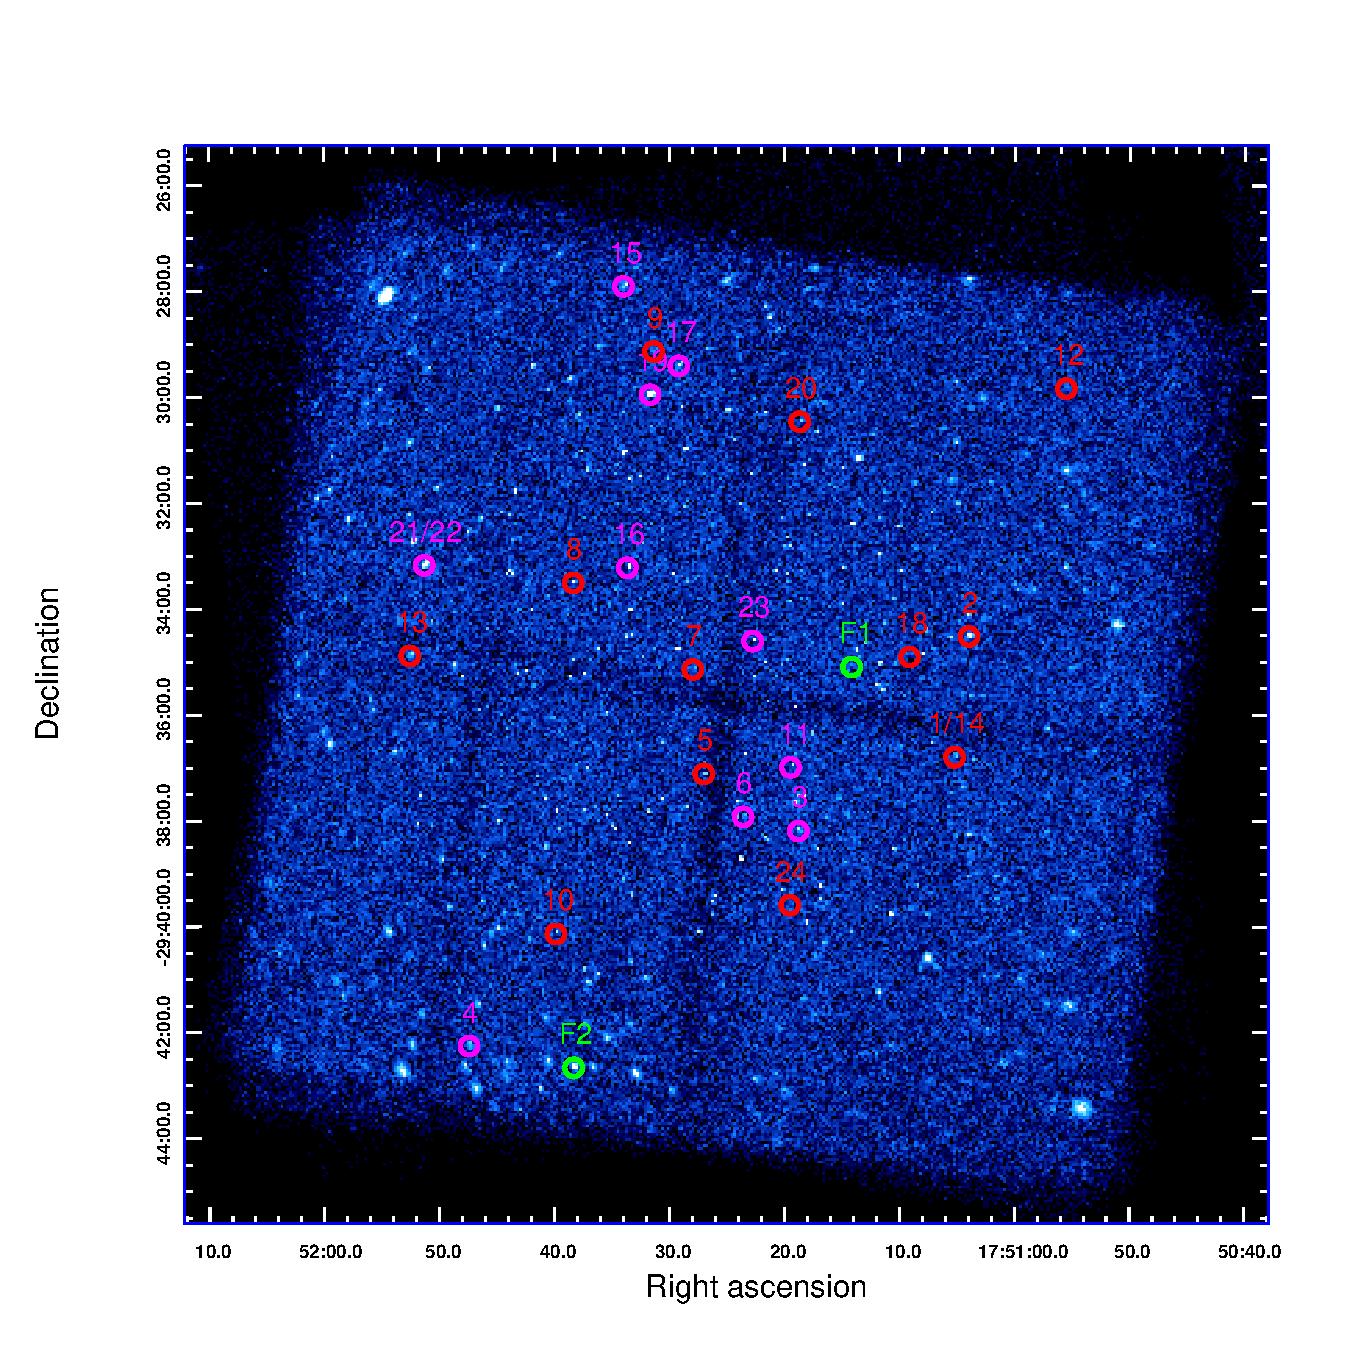
\includegraphics[scale=0.8]{./figure/LW/all_pCVf.eps}
\caption{2--8 keV counts image of the Limiting Window, combining 13 {\it Chandra}/ACIS-I observations. Locations of the 24 periodic sources are marked with colored circles ({\it magenta}: 10 sources previously reported by \cite{2012ApJ...746..165H}; {\it red}: 12 newly discovered in this work and belonging to the Galactic bulge; {\it green}: two newly discovered and located in the foreground). Source numbering is the same as in Table~\ref{tab:src}.}
\label{fig:FoV}
\end{figure*}

\section{Period Searching Method}\label{sec:methods}
In this section, we first provide our motivation of employing the Gregory-Loredo (GL) algorithm, followed by a description of its basic principles (Section~\ref{subsec:GL}). We then elucidate our application of the GL algorithm to the {\it Chandra} data of the LW (Section~\ref{subsec:appli}). This is complemented by a set of simulations to evaluate the detection (in)completeness (Section~\ref{subsec:simulation}).  

\subsection{The Gregory-Loredo Algorithm} \label{subsec:GL}
There exists in the literature a variety of period-searching methods, which can be broadly divided into three categories according to their working principles. 

The most traditional method is based on Fourier transform and its power density spectra, which includes the classical Schuster periodogram \citep{1898TeMag...3...13S}, the Fourier analysis with unequally-spaced data \citep{1975Ap&SS..36..137D}, the correlation-based method \citep{1988ApJ...333..646E}, among others.

Another widely-used method seeks to fit the data with a periodic model in the frequency space, employing statistics such as least-squares residuals to define the likelihood function and then selecting the frequency that maximizes the likelihood. The famous Lomb-Scargle periodogram \citep[hereafter LS]{1976Ap&SS..39..447L,1982ApJ...263..835S} belongs to this category. Note that when adopting trigonometric functions, the least-squares method falls into the Fourier method. Another variant is to replace the least-squares residuals with polynomial fits, such as that used in \citet{1996ApJ...460L.107S}.

The last category is the phase-folding method. For each trial period the time-tagged data is folded as a function of phase, and the best-fit period is found by optimizing the cost function through the frequency space. Cost function are designed  to evaluate how much the phase-folded light curve deviate from constant.
Methods belonging this category use diverse cost functions. Several widely known examples are the Epoch Folding (EF) algorithm \citep{1983ApJ...266..160L}, the Phase Dispersion Minimization \citep{1978ApJ...224..953S}, the GL algorithm \citep{1992ApJ...398..146G}.

In X-ray observations, the detection of periodic signals is often involved with irregularly and sparsely sampled data. The relatively few detected photons makes it inappropriate for the first two groups of methods since they need photometric data. Though we could choose a length of time bin to covert the event data to photometric data, the small number of photons makes lower signal-to-noise ratio when using time bins. Fortunately, the phase-folding methods directly manipulate each photons and thus keep the full information from observation. Another characteristic for astronomical observation is the interrupted time series. In frequency space, this kind of window function leads to the heavy contamination for intrinsic data. Still, the phase-folding methods can avoid the effect of non-uniformed data since the process does not contain information in non-observed time. 

Considering the above, here we use GL method to find periodic signals. GL method applies the Bayesian probability theory to the cost function. We would make a brief overview about Bayes's theorem and the identification of periodic signals in GL method in appendix \ref{GL}. The key of this algorithm is the multiplicity of the binned distribution of events. 
\begin{equation}\label{multi}
W_m(\omega, \phi)={{N!}\over{n_1!\; n_2!\; n_3!\cdots {n_m}!}}
\end{equation}
$N$ represents the total number of counts in data, $m$ signifies the number of bins. $n_i(\omega, \phi)$ is the number of events falling into the $i$th of m phase bins by given the frequency $\omega$ and the phase $\phi$, where $\sum\limits_{i=1}^{m}n_i(\omega, \phi)=N$. For the data of N counts, the model defined by $\omega$ and $\phi$, the multiplicity is the number of ways that the distribution could have arisen by chance. The probability of periodic is inversely proportional to the multiplicity. It could be easily proved that when the value of $n_i$ are far apart, the multiplicity is reduced to a lower value. In simpler terms, the more the stepwise model deviate from constant, the higher the signal is periodic. 

In general, firstly we got the multiplicity for all the set of $(m,\omega, \phi)$. secondly, the integration was applied in $(\omega, \phi)$space, producing the so-called "odds ratio" using Bayesian theorem when m took a certain value. Thirdly, the probability of whether the dataset is periodic was obtained by the sum of normalized odds ratio. Finally, comparing all the odds ratio integrated at only $\phi$ space, the $\omega$ with the highest odds ratio, corresponding the period of signal.

%\section{Period searching procedure}\label{sec:timing}
\subsection{Application to the LW}\label{subsec:appli}
Though we did source detection in 2-8 keV band to reduce the contamination from non-CV sources, here we still extracted photons from sources in 1-8 keV band to keep as more as possible source information. 
Besides, in order to compensate for uneven distribution over the bins, we provide "epoch" for each source. The "epoch" offered the start time and end time of each observations covered the source with at least one counts in source region. See Eqn.~\ref{A17} \textcolor{red}{always add Eqn. when quoting equations} in appendix for detailed illustration about the use of epoch. 
For the sake of changing aimpoint, we used individual source extract region for different observations. Explicitly, the 90\% ECR aperture  whose radius defined by specific PSF map was applied for counts in that observation. Since the phase-folding method directly manipulated each photons and we could not distinguish background photon from source photon, the local background information were not provided for timing analysis. The combination of each source event list and the corresponding epoch were then employed as the input of GL method. 
\\
\indent
As mentioned in section \ref{subsec:GL}, the GL method fold the dataset at trial period or frequency. Then the resolution of frequency must be balanced between computational power and  accuracy. Here we generate the frequency resolution depended on the data timescale.
\\
\indent
For the data span in timescale T, the arrival time of photon $t_i$, the changing angular frequency influence the phase of photon more as $i$ grows. The most vulnerable photon is the last photon arrived, whose arrival time is T, and the change of phase is 

\begin{subequations}\label{fi}
\begin{equation}
	d\phi_{N}=\phi_{N}^{'}-\phi_{N}
\end{equation}
\begin{equation}
	\phi_{N}^{'}=(\omega +d\omega) \cdot T-\lfloor (\omega +d\omega) \cdot T \rfloor
\end{equation}
\begin{equation}
	\phi_{N}=\omega \cdot T-\lfloor \omega \cdot T \rfloor
\end{equation}
\end{subequations}
\\

Assuming $\lfloor (\omega +d\omega) \cdot T \rfloor = \lfloor \omega \cdot T \rfloor$, ($\lfloor a \rfloor$means the integral part of a), then 
\begin{equation}
	d\phi_{N}=d\omega \cdot T
\end{equation}
In this work, we take 12 as the largest number of phase bins, that demands the change of photon phase should be smaller than ${1\over 12}\cdot 2\pi $ to guarantee the nearly non-change of phase-folded light curve. Although we can not ensure every photon to meet the requirement since its location in the same phase bin could be arbitrary. It would satisfy the situation at nearly perfect level if we keep the deviation of phase of last photon smaller than ${1\over 12}\cdot 2\pi $. As shown in equation \ref{dfi}
\begin{subequations}\label{dfi}
\begin{equation}
	d\phi_{N}=d\omega \cdot T< {1\over 12}\cdot 2\pi
\end{equation}
\begin{equation}
	d\omega < {{\pi}\over {6\;T}}
\end{equation}
\end{subequations}

The total span of 13 observation is about three years, i.e., $10^8s$, so the resolution of angular frequency is $5\times 10^{-9}$. When the $\omega$ increases, corresponding the period decreases, the same resolution brings numerous discrete frequencies and raises running time greatly. Thus we used three different resolutions $10^{-7},10^{-8},10^{-9}$ in three period ranges $(300s,3000s),(3000s,10000s), (10000s,50000s)$. The ranges was chosen for the orbital period distribution of CVs, as shown in Figure \ref{fig:N_P}. There is a period gap in distribution at 2-3 hours, and a period minimum at about 70 minutes. Then the first range covers roughly the spin period of IPs, the other two ranges overlay the orbital period below and beyond the period gap respectively.

Generally, for each source, we provide the dataset for GL method. Then we got the most periodic signal with its probability in three period ranges. Taking 90\% as threshold to determine the periodicity, finally we choose all the candidate sources with at least one periodic signal.

\subsection{Detection completeness}\label{subsec:simulation}
For a given period searching algorithm, the detection rate depends on both the number of observed counts and the intrinsic shape of light curve.
We perform simulations to quantify the detection rate, following the merit of \citep{1998ApJ...498..666C}. 
Two functional forms of light curve are considered: a sinusoidal function and a piecewise function. While these are idealized shapes, they can represent realistic light curves, e.g, resulted from rotational modulation or eclipsing. 

A sinusoidal light curve follows,
\begin{equation}
\lambda (t)=\lambda_0[1+A_{0}{\rm sin}(\omega t+\phi)], 
\label{eqn:sin}
\end{equation}
where $\omega = 2{\pi}/P$ is the frequency, $A_0$ the variation amplitude, and $\lambda_0$ the mean count rate which may include contribution from a constant background. 
For a direct comparison with the observation, we replaced $\lambda_0$ with the total number of counts, $C = \lambda_0 T$, where $T$ is the exposure time of a given observation. This holds since $T$ is typically much longer than the modulation period ($P$). 
%Since the limit of computational power, the simulation were run at limited numbers of parameters. 
We casually chose three period in different period ranges, which was 554, 5540 and 45540 sec. The values were not chosen by any physical reasons. These three period represent the performance of GL method in three period ranges. 

The simulation is operated with counts(cts=$50-500$), amplitudes($A_0$=$0.5-0.9$), period(P=$554s,5540s,45540s$). The top, middle, bottom panel of Figure \ref{fig:detection} show the results of three period respectively. For each set of parameter, the GL method were run on 100 sinusoidal light curves.
The valid detection of GL method need to constrain the period at 0.1\% accuracy and get periodical probability beyond 90\%.
The detection rate is the proportion of the number of valid detections in one hundred.

\begin{figure}[htbp]
\gridline{\fig{./figure/sim_LW/detection_554_temp.eps}{0.45\textwidth}{}}
\gridline{\fig{./figure/sim_LW/detection_5540_temp.eps}{0.45\textwidth}{}}
\gridline{\fig{./figure/sim_LW/detection_45540_temp.eps}{0.45\textwidth}{}}
\caption{Detection rate obtained from simulation results for sinusoidal variation. The results of top, middle, bottom are respectively from modulation period as 554s, 5540s, 45540s. The other two parameters, $A_{0}$ and number of counts, are labeled by x-axis and colors. \label{fig:detection}}
\end{figure}
We could think of 0.1 as extremely low. Then it is obviously illustrated that when counts equals 50, the detection rate are almost always extremely low despite the period and amplitude, except for the longest period and high amplitude. While for counts of 100, the detection rate could invariably exceed 50\%, which is sufficient enough for period finding procedure. Thus we could roughly say that when counts lower than 100, the detection rate is extremely low. The periodic signal in this circumstance are not reliable. Besides, it can be seen that the algorithm is nearly no bias of period, except a slight improvement of detection rate with increasing period.
 
The piecewise function, which mimics an eclipse against an otherwise constant flux, takes the form of

\begin{equation}
\lambda(t)=
\begin{cases}
\lambda_0 & \text{$\phi(t)/2\pi \in[0,{{1-w}\over{2}})\cup ({{1+w}\over{2}},1]$},\\
f\lambda_0 & \text{$\phi(t)/2\pi \in[{{1-w}\over{2}},{{1+w}\over{2}}]$},
\end{cases}	
\end{equation}
where $w$ accounts for the eclipsing width (duration) in phase space, and $f$ characterizes the fractional depth of the eclipse, with $0\leq f \leq 1$. Here the eclipse is assumed to occur around $\phi = \pi$.

We took $f=0.1$, $w=0.1$ as constant, in order to obtain the relation between detection rate and number of counts. These two values are really typical for the case of CV, since the radius ratio of WD, companion star and orbit are about   1:10:50. The relation between counts number N and $\lambda_0$ is $N=(1-0.1*0.9)\lambda_0T$.
The period was also chosen causally, at P=5258s and P=15258s. Then the simulation were run 100 times at each set of parameter. Results of detection rate(also taking 90\% as threshold) is shown is Figure \ref{fig:eclipse}. It is noteworthy that the efficiency soars to 1 when the number of counts goes up. And a marked rise appears with the growth of period.
 
\begin{figure}[ht!]
\centering
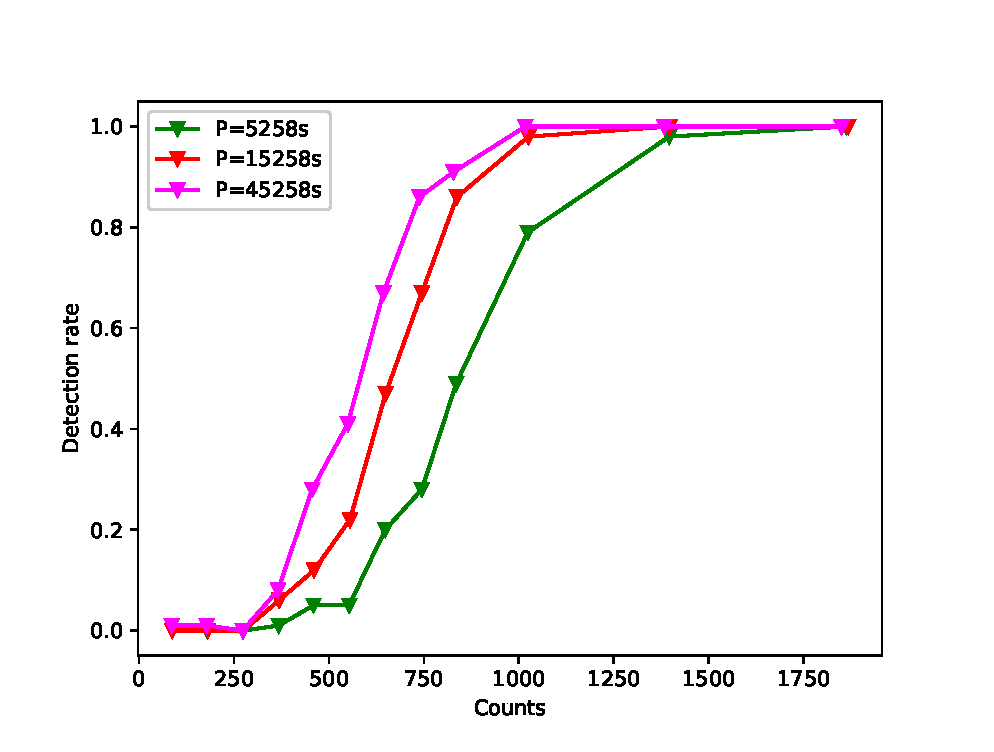
\includegraphics[scale=0.61]{./figure/sim_LW/eclipse.eps}
\caption{Detection rate obtained from simulation results for eclipsing models. Red and green denotes for P=15258s and 5258s respectively. \label{fig:eclipse}}
\end{figure}


%  \subsection{Long timescale variability}\label{longT}
% For the purpose of comprehending the non-periodic variability of these periodic sources, we quantified the 1-8 keV flux variation among all the 13 observations. We employed the CIAO tool \emph {aprates}, which uses Bayesian statistics to compute the source intensities including net counts, photon flux and their confidence bounds. The source extract region was the same aperture as the input of GL method, i.e., 90\% ECR. The background region was chosen to be an annulus with inner-to-outer radii of 2 and 4 times the 90\% ECR. To avoid the contamination of nearby point sources and extended sources, we double-checked this background region by eyes and exclude these contaminated region. Note all the radius is determined by individual PSF map. We took 3$\sigma$ limits to define the detection. If the 3$\sigma$ lower limit beyond zero, then this observation had a valid detection. For non-detection observation, we only presented its upper limit. Additionally, we defined $VI=S_{max}/S_{min}$ to indicate the variability, where $S_{max}$ and $S_{min}$ is the maximum and minimum photon flux among all the valid detection over 1-8 keV band.
% \\
% \indent
% The long timescale variability analysis was only applied for the preliminary results of GL methods, i.e., the candidate periodic sources, since the time limit resulted from visual examination for regions.

\section{Period Searching Results}\label{sec:results}
\subsection{Filtering detections}
From period searching by GL method and taking 90\% as threshold, we got 73 periodic signals in three period ranges. The spurious detections are severe, resulted by many reasons.
\\
\indent
(1) There are repetitious detection for the same intrinsic signal caused by second and third harmonics. Luckily, it's easy to identified by phase-folded light curves If we assume that it's a single-peak structure. We had to assume that there was no half harmonics and took the lowest period signal as the real period. Discussion about harmonics would be detailed below in section \ref{harmonics}. 
\\
\indent
(2) The Chandra satellite was designed with dithering to distribute photons over more CCD pixels and avoid pile-up effect. The dither period is about 706.96s in pitch and 999.96s in yaw. All signals around these two and their harmonics were excluded, which happened most in the first period range.
\\
\indent
(3) The strong outburst in long timescales would confuse the GL method since this algorithm directly analyzed the phase folded light curve. If there are too many photons in one of the observations, some phase bins would show unusual excess at long period. Then the method may "think" there is a period of the source especially in the third period range. Therefore, the periodic sources with VI>10 were excluded. 
\\
\indent
(4) The foreground sources is not of our interest. Meanwhile, the uncertainty of their distances resulted the unknown luminosity, which increased the confusing part of their nature. We applied the spectral fitting results to distinguish them from galactic bulge sources. If the absorption column density (hereafter $N_{H}$) is lower than $5 \times 10^{21} cm^{-2}$, it would be taken as foreground source. Though they are not spurious but valid detection, we only present their period and coordinates in Table \ref{tab:src} labeled by F1 and F2, without further discussion.
\\
\indent
(5) We took N=100 as the search limit based on the simulation results. The sources whose number of counts are lower than 100 were ignored. The choice for this limit has been explained explicitly in section \ref{simulation}. The choice served as compensation for the third filtering. Due to the nearly no valid detection for faint sources, we were incapable to give VI for them following the routine of section \ref{longT}. Although we could not obtain the false-detection rate (i.e. reliability) from simulation cause of no unified long timescale variability model. It was still trustworthy to assume the higher false-detection rate for fainter sources. Collectively, we exclude the detection signal for sources under that limit. 
\\
\indent
After these limitations were applied, we got 24 valid detection of periodic signal in 22 sources. Two of these sources showed two period in different period ranges.
\subsection{Treatment of harmonics}\label{harmonics}

To determine the intrinsic period, whether it's rotation period or orbital period, from primary period and harmonics, we should not focus on data and the significance of signals. In that the intensities of signals could not reflect the authenticity of the signal precisely. For the sake of  identification, the physical mechanism of period in CVs must be introduced. 

Here we take the 6th signal as an illustration, the phase-folded light curve of primary period and second harmonic show classic  single-peak shape and double-peak shape, see the left two panels in Figure \ref{fig:6thfig}. For comparison, we also present the phase-folded light curve of J1817-2508 based on XMM-Newton observations (obsID=0601270301).

 The J1817-2508, which was also called IGR J18173-2509, has been determined with pulsation at 830.70s from Swift-XRT detection. Then the signal of 1660s has also been detected from Chandra observation \citep{2009ATel.2354....1N} and the optical period of 1690s \citep{2012A&A...542A..22B}. All the above strongly suggests that the true spin period is about 1660s, twice the first detected X-ray period, even though the two peaks in modulation are quite similar, as shown in the lower right panel in Figure \ref{fig:6thfig}.
 
 The properties of J1817-2508 indicates that phase-folded light curve could be extremely deceptive under the circumstances that sources with symmetric dipole structure. We could not precisely determine the true rotation period without optical observations. However, the physical origins of periodic signals may provide additional constrains on the judgement. The double-peak shape only happens in IP with accretion column model. The two poles where accretion region lied on, would be the brightest. When we look at them at a specific angle, the two poles alternatively flitting across the face of WDs, and then produce the double-peaked pulsation. In this kind of situation, the modulation period must be the rotation period of WDs, mostly under one hour. While the second harmonics of our sources, are mostly beyond 3 hours. It would be a risky assumption if these harmonics served as spin period. On the other hand, despite the WDs in polars may have such long rotation period from synchronization effect, their accretion stream always falls on the single pole, emitting most of the soft X-ray radiation. Then the double-peaked pulsation are almost impossible. 
 
 In conclusion, according to the length of period in our sources, we took the single-peaked signal, normally the shortest period, as the real orbital period. The double-peaked shape in harmonics are treated as spurious signal. 


\begin{figure*}[htbp]
\gridline{
\fig{./figure/LW/pfold_lc_20.eps}{0.45\textwidth}{}
\fig{./figure/CV/pfold_lc_J1817_2508_spin_half.eps}{0.45\textwidth}{}
}
\gridline{
\fig{./figure/LW/pfold_lc_20_second.eps}{0.45\textwidth}{}
\fig{./figure/CV/pfold_lc_J1817_2508_spin.eps}{0.45\textwidth}{}
}
\caption{The top left and bottom left panel show the folded light curve of LW 6, at true period and second harmonics, respectively. The top right and bottom right panel display the folded light curve of J1817-2508. While for this source, the double-peaked shape (bottom right) at 1660s are the real signal of rotation. \label{fig:6thfig}}
\end{figure*}

\begin{figure*}[htbp]
\centering
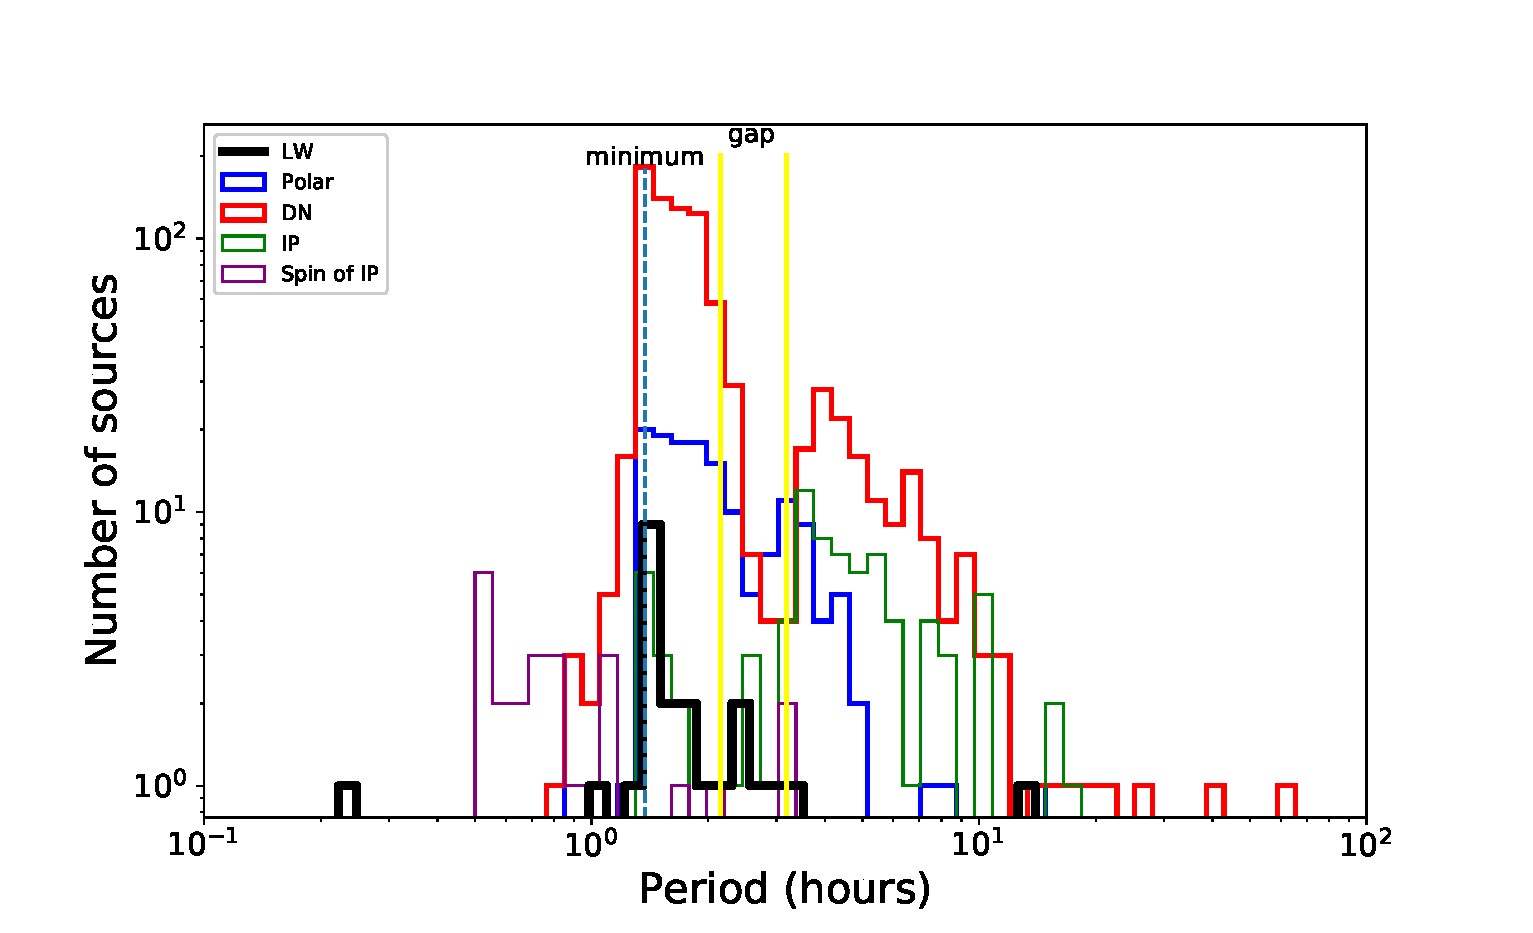
\includegraphics[scale=0.73]{./figure/CV/N_P.eps}
\caption{The period distribution of the LW sources (dark-blue line), the spin (purple) and orbital (green) periods of IPs ,the periods (sky-blue) of polars and the orbital (red) periods of DNe from the RK catalog(\cite{2003A&A...404..301R}, version 7.20). The famous period gap(yellow line) and period minimum(orange dashed line) are also plotted, whose value are taken from \citep{2011ApJS..194...28K}.\label{fig:N_P}}
\end{figure*}

\subsection{Results}
For the 24 signals, their phase-folded light curve at modulation period, the long-term light curve and spectra are shown in Figure \ref{fig:Figure_p}, sorted by the order of increasing period. 

For left panel, though the GL method could not distinguish background photons, we still define the local background from photometric results, shown as the yellow strip in the left panel of Figure \ref{fig:Figure_p}. The width of strip represents the poisson error range.
Additionally, since the bin size in phase-folded light curve has no effect on the shape, we chose the bin size between 20 to 50, to get the most distinct display. 
For middle panel, the valid detection (defined in \ref{longT}) are plotted with dots plus error range. While the non-valid detection are shown in arrows, providing only the upper limits. Meanwhile, the x-axis in right panel were plotted in discontinuous style for better demonstration effect, since the short interval over the last eight observations. 
For right panel, the spectra illustrated here were fitted in the range of 1-8 keV, consistent with the timing analysis. 
\\
\indent
Besides, we also did 100 times of simulations for each signal. We had to use sinusoidal variations for simulating process though many of them may deviate much from real shape. The counts rate and period can be directly attained from data, while the amplitude is hard to determine since the deviation. In \citet{2012ApJ...746..165H}, they defined $A_{M}={1-R_{min}}/R_{max}$, and $A_{M}=2A_0/{1+A_0}$, where $R_{min}(R_{max})$ is the minimum (maximum) count rate of the folded light curve. 
Though the $A_{M}$ depends on the bin size of phase-folded light curve, we still prefer it rather than $A_{rms}$ to get the amplitude since the deviation between sinusoidal variation and real shape sometimes made $A_{0}$ exceeds one when it was calculated from $A_{rms}$. The definition of $A_{rms}$ and the relation between 
$A_{rms}$ and $A_0$, which were taken by \cite{2012ApJ...746..165H}, are described below.
\begin{subequations}
\begin{equation}
A_{\mathrm{rms}}=\left(\frac{Z_{1}^{2}}{N}\right)^{1 / 2} \frac{N}{N-B}
\end{equation}
\begin{equation}
Z_{1}^{2}=\frac{2}{N}\left\{\left[\Sigma_{j} \cos \phi\left(t_{j}\right)\right]^{2}+\left[\Sigma_{j} \sin ^{2} \phi\left(t_{j}\right)\right]^{2}\right\}
\end{equation}
\begin{equation}\label{Arms}
A_0=\sqrt{2} A_{\mathrm{rms}}
\end{equation}
\end{subequations}
where equation \ref{Arms} only works for sinusoidal modulations. N and B represent the total counts in source region and local background respectively. $t_{j}$ and $\phi\left(t_{j}\right)$ refer to the arrival time and phase of each photon. $Z_{1}^{2}$ is the classical Rayleigh statistic method \citep{1983A&A...128..245B,2003ApJ...599..465M}.

Still, we took 90\% as threshold to get valid detection at 0.1\% accuracy. The percentage of valid detection would be represented by $P_{det}$. And $A_{M}$ was obtained with bin size fixed at 20.

The periodic sources and their information are shown in Table \ref{tab:src}, which also includes the cross-match results with \cite{2012ApJ...746..165H}. The ten periodic sources discovered by \cite{2012ApJ...746..165H} have also been determined by GL method in this work.

\begin{deluxetable*}{LCCCCCCCCCCC}
%\tablenum{2}
\tablecaption{Periodic sources and information in LW \label{tab:src}}
\tablewidth{0pt}
\tablehead{
\colhead{ID} & \colhead{R.A.} & \colhead{Decl.} &
\colhead{Period} & \colhead{H-ID} & \colhead{Counts} &\colhead{$A_0$} &\colhead{H-$A_0$}& \colhead{$P_{det}$} & \colhead{H-$P_{det}$} &\colhead{$P_{det}'$} & \colhead{Notes}\\
\colhead{LW} & \colhead{$\circ$} & \colhead{($\circ$)} & 
\colhead{(s)} & \colhead{} & \colhead{1-8 keV} & \colhead{} & \colhead{} &\colhead{\%}  &\colhead{\%} &\colhead{\%} &\colhead{}
}
\decimals
\decimalcolnumbers
\startdata
1^\dag & 267.77173 &	-29.61332 & 853.83 &-& 202 & 0.76  &-& 86 &-&-&- 
\\
2 & 267.76657 &	-29.57529 & 3820.83 &-& 902 & 0.54 
	&-& 99 &-&-&-
\\
3 & 267.82829 &	-29.63660 & 4728.90 & H6 & 394 & 0.75 & 0.71 & 98 & 80.1 & 99 & \text{Third}
\\
4 & 267.94766 &	-29.70427 & 4886.79 & H8 & 784 & 0.56 & 0.57 & 100 & 9.6 & 98 &- 
\\
5 & 267.86255 &	-29.61859 & 5072.97 &-& 293 & 0.76 &-& 100 &-&-& \text{Second}
\\
6 & 267.84831 &	-29.63212 & 5130.57 & H2 & 437 & 0.76 & 0.83 & 100 & 99.9 & 100 & \text{Second}
\\
7 & 267.86651 &	-29.58575 & 5144.97 &-& 335 & 0.77 &-& 100 &-&-& \text{Second}
\\
8 & 267.90982 &	-29.55845 & 5158.75 &-& 121 & 1.00 &-& 100 &-&-& \text{Second}
\\
9 & 267.88075 &	-29.48562 & 5231.49 &-& 347 & 0.67 &-& 100 &-&-&-
\\
10 & 267.91616 &	 -29.66900 & 5252.93 &-& 211 & 0.83 
	&-& 100 &-&-&-
\\
11 & 267.83116 &	 -29.61651 & 5261.93 & H10 & 438 & 0.88 & 0.42 & 100 & 13.9 & 31 & \text{Second}
\\
12 & 267.73141 &	 -29.49721 & 5334.76 &-& 760 & 0.51 
	&-& 100 &-&-& \text{Second}
\\
13 & 267.96901 &	 -29.58142 & 5501.16 &-& 512 & 0.61 
	&-& 100 &-&-&-
\\
14^\dag & 267.77173 &	 -29.61332 & 5608.21 &-& 202 & 0.81 &-& 100 &-&-& \text{Third}  
\\
15 & 267.89161 &	 -29.46508 & 6335.85 & H5 & 823 & 0.62 & 0.61 & 100 & 67.5 & 100 & \text{Second} 
\\
16 & 267.89024 &	 -29.55369 & 6597.55 & H9 & 487 & 0.72 & 0.55 & 100 & 66.1 & 99 & \text{Second}
\\
17 & 267.87162 &	 -29.49011 & 7448.98 & H3 & 535 & 0.73 & 0.92 & 100 & 99.1 & 100 & \text{Second}
\\
18 & 267.78806 &	 -29.58177 & 7756.19 &-& 214 & 0.91 &-& 98 &-&-& \text{Second}
\\
19 & 267.88203 &	 -29.49922 & 8546.28 & H4 & 3402 & 0.30 & 0.20 & 99 & 83.3 & 93 & \text{Second}
\\
20 & 267.82785 &	 -29.50770 & 8844.82 &-& 263 & 0.69 
	&-& 93 &-&-& \text{Second}
\\
21^\ddag & 267.96375 &	 -29.55290 & 9877.52 &-& 1963 & 0.40 &-& 100 &-&-&- 
\\
22^\ddag & 267.96375 &	 -29.55290 & 10342.30 & H1 & 1963 & 0.76 & 0.37 & 100 & 99.8 & 99 &-
\\
23 & 267.84487 &	 -29.57680 & 12002.70 & H7 & 307 & 1.00 & 0.85 & 100 & 25.7 & 100 & \text{Second}
\\
24 & 267.83142 &	 -29.65992 & 47317.12 &-& 138 & 0.88 
	&-& 87 &-&-&-
\\
\hline
\hline
F1 & 267.80902 &	 -29.58494 & 39636.93 &-& 169 &-&-&-&-  &-&-
\\
F2 & 267.90974 &	-29.71112 & 42219.03 &-& 1039 &-&-&-  &-&-&-
\enddata


\tablecomments{Columns:
\\(1) Source sequence number assigned in the order of increasing period. The same source with multiple period signal was denoted as \dag and \ddag. F1 and F2 represent the two periodic foreground sources.
\\(2) R.A.(J2000) of the centroid of source. 
\\(3) Decl.(J2000) of the centroid of source. 
\\(4) The modulation period determined by GL method.
\\(5) The cross-match results with previous work. $H_{i}$ represents the $i$th source in Table 2 of \cite{2012ApJ...746..165H}. 
\\(6) The number of counts in the 1-8 keV band. 
\\(7) The amplitude of variation obtained in this work. 
\\(8) The amplitude of variation obtained in \cite{2012ApJ...746..165H}. 
\\(9) The detection probability of periodicity based on simulations of 100 sinusoidal light curves for each source.
\\(10) The detection probability of periodicity in \cite{2012ApJ...746..165H}.
\\(11) The detection probability of periodicity simulated as the same process described in column(9), while the amplitude are taken from column(8).
\\(12) The note gives the significant harmonic detected by the algorithm.
}
\end{deluxetable*}

\section{X-ray spectral analysis}\label{sec:spectra}
For all candidate periodic sources, we employed the same region as described in section \ref{longT} and combined the individual spectra together by using the CIAO tool \emph {specextract}. Then we made the spectra analysis in XSPEC v12.9.1 over the range of 0.5-8 keV. The adaptive binning had been conducted before the fitting with signal-to-noise ratio of 2. The reason we present the fitting results of 0.5-8 keV here is to constrain the absorption. Notice that the choice of energy range is not consistent with the illustration of spectra in Figure \ref{fig:Figure_p}, even though it has little impact on exhibition. 
\\
\indent
We modeled the spectra by using a bremsstrahlung continuum plus three Gaussian lines centered at 6.40, 6.68 ,and 6.97 keV respectively  \citep{2018ApJS..235...26Z,2019ApJ...882..164X}. And all these model components are multiplied by an absorption component(using the model \emph {phabs} in XSPEC). The spectral analysis results are shown in Table \ref{tab:spec}.
\\
\indent
The plasma temperature could not be well constrained caused by the intrinsic hard spectrum and the bad sensitivity of \emph{Chandra} above 8 keV. Hence we fixed $T_b$ at 40 keV under the not-constrained situation, which is the typical value of IPs \citep{2016ApJ...826..160H}.
Besides, we provided the information of Fe K emission line, which had been proved as the great probe of the mass of white dwarfs in CVs \citep{2016ApJ...818..136X}. The flux ratio of Fe XXVI to Fe XXV emission lines (hereafter $I_{7.0}/I_{6.7}$) could be interrelated to the $M_{WD}$ by uniting the $I_{7.0}/I_{6.7}$-$T_{max}$ and $T_{max}-M_{WD}$ relations \citep{2019ApJ...882..164X}. Due to the low metallicity in LW field, most of sources in our table have weak emission of iron line. We employed the XSPEC tool \emph{multifake} to derive the confidence range of $I_{7.0}/I_{6.7}$ and $I_{6.4}/I_{6.7}$. Then we excluded the source whose 68.3\% confidence range for the intensities of three iron lines are all below zero. After the filtering process, we only got 2 sources with valid detection of at least one iron lines. The value of flux ratios are presented together with their 68.3\% confidence range (see column (4) and (5) in Table \ref{tab:spec}). Referring to the $I_{7.0}/I_{6.7}$-$M_{WD}$ relation in \citet{2019ApJ...882..164X}, the WD mass of LW 21(or LW 22) and LW 23 would be around 0.8 and 0.5 $M_\odot$ if they are IPs, or 1.2 and 1.0 $M_\odot$ if DNe, respectively.

We divided the 22 periodic sources into two groups based on their luminosities obtained above. H(L) sources included the sources having 1-8 keV luminosity above(below) $\rm 1 \times 10^{32}~erg ~s^{-1}$. The number of sources in these two set were 6 and 16 respectively. Their cumulative spectrum were fitted with the same model for individual sources. And the best-fit results are presented in Table \ref{tab:pCV_spec}. The H and L spectra are shown in Figure \ref{fig:pCV_spec} over the energy range of 0.5-8 keV. Using the XSPEC tool \emph{multifake}, we have gotten well constrained line ratios for this two subtypes. Cosulting the $I_{7.0}/I_{6.7}$-$M_{WD}$ relation in \citet{2019ApJ...882..164X}, the H sources have mean $M_{WD}$ about 0.8(1.2) $M_\odot$ if they are IPs (non-mCVs). The $M_{WD}$ of L sources would be lower than 0.4 $M_\odot$ suppose they are non-mCVs. However,we have no reliable relation for polars.


%% Appendix material should be preceded with a single \appendix command.
%% There should be a \section command for each appendix. Mark appendix
%% subsections with the same markup you use in the main body of the paper.

%% Each Appendix (indicated with \section) will be lettered A, B, C, etc.
%% The equation counter will reset when it encounters the \appendix
%% command and will number appendix equations (A1), (A2), etc. The

\section{The properties of X-ray periodic sources}\label{sec:properties}
It can be seen that the luminosities of these periodic sources are ranged from $\rm 10^{31}$ to $\rm 10^{33}~erg~s^{-1}$, combined with the period distribution, mostly about 1-3 hours , all suggest that they belong to cataclysmic variables. 
Before we start to discuss the nature of these periodic sources, we should take a look at CVs in the field. Their period distribution, including polars, IPs and DNe, are shown in Figure \ref{fig:N_P}.
It can be easily seen that the period distribution of these LW sources resembles those of polars more than others, since most of these are below the period gap. While DNe and IPs both have a considerable number of systems with period beyond the gap. According to the our simulation results in section \ref{simulation}, this can not be resulted from selection bias of algorithm. 

For non-magnetic CVs like DNe, the common phase-folded light curve exhibits narrow dip, due to the eclipse of the white dwarf, as modeled in section \ref{simulation}. The typical light curve is like \#22 in Figure \ref{fig:Figure_p}. 	While the simultaneous existence of \#21 and \#22 and the 2\% period difference suggest it might be an asynchronous intermediate polar. Besides, the central dip of \#3, \#18 and \#20 are also similar to this circumstance. Since the eclipse happens in nearly all types of CVs, we could only set three as an upper limit of number of DNe in our sample.

For magnetic CVs, including IPs and polars, their orbit modulation could give rise to more complicated shape of light curve. For polars, consider the simplistic situation, whose accretion is nearly onto one pole, then the shape of light curve would be divided into two groups. Suppose an inclination $i$, the angle between rotation axis and magnetic axis is $\beta$, the magnetic colatitude of accretion is $\epsilon$. Then if $i+\beta+\epsilon > 90^{\circ}$, we would see alternately two poles, the shape would be like \#6, with half of orbit cycle showing no emission. This so-called "two-pole"  behavior are more complicated if the accretion goes to both two poles, the gap with half orbit cycle would be partially filled (like \#16) by second pole's emission. Sometimes it may completely reverse in hard X-ray band cause the accretion shock in second pole producing most of hard X-rays \citep{1985A&A...148L..14H}. On the other hand, if $i+\beta+\epsilon < 90^{\circ}$ and $\beta < i$, in which the accreting pole is always visible , the modulation would caused by the obscuring of accretion stream. The width and depth of the dip in phase space are determined by many reasons and totally unpredictable. 

For IPs, the orbital modulation could be resulted by eclipse of WD, the absorption of X-rays emitted near the white
dwarf surface \citep{1993MNRAS.260..299H}, or the "disc-overflow" model in \citep{1996MNRAS.280..937N}. The shape of light curve in IPs could be any kinds of dips or sinusoidal variation. The only robust identification is to determine both their spin and orbital period, like the \#1(\#14) and \#21(\#22) in our sample.

Based on our current understanding of the shape and distribution of orbital modulation, we conclude that the periodic sources discoverd are mostly polars, with several IPs(two determined) and DNe(three as upper limit). 

\section{Discussion}\label{sec:discussion}
\subsection{Comparison with previous work}
In this work, we took the same observations as used by \cite{2012ApJ...746..165H}. However, unlike \cite{2012ApJ...746..165H} extracted only the some nearby observations , all the observations were applied here for timing analysis. That difference was caused by the mechanisms of methods. As described in section \ref{subsec:GL}, the LS method used by \cite{2012ApJ...746..165H} handled the light curve in time space, while GL method utilized here  processed the phase-folded light curve in phase space with great tolerance for observing gap.

 We provide the comparison between the detection rate of these two methods in Figure \ref{fig:com}, which are also shown in column (10) and (11) in Table \ref{tab:src}. To eliminate the effect of different choice of amplitude for the same source, we used the same $A_0$ of these ten sources given by \cite{2012ApJ...746..165H} and applied these to both methods. It can easily be seen that GL method has better performance compared with LS method.

The improvement on detecting efficiency and data usage brought more periodic signals than \cite{2012ApJ...746..165H}. Additionally, we operated the simulation not only for sinusoidal variation, but also for eclipsing models to describe the dip in orbital modulation. Combining the simulation results and more than twice the sample, we were allowed to discuss the source properties and the distribution of CVs in galactic bulge region on a better level.

\begin{figure}[htb]
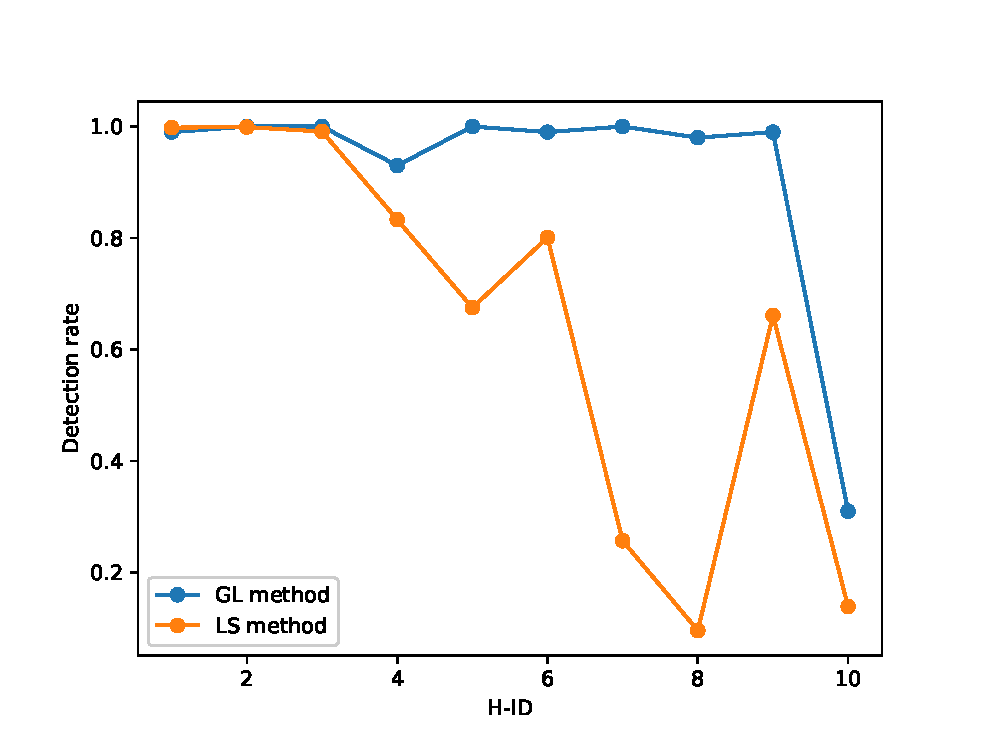
\includegraphics[scale=0.55]{./figure/sim_LW/Pdet_com.eps}
\caption{The comparison of efficiency between two methods. H-ID is the sequence number given by \cite{2012ApJ...746..165H}, same as column(5) in Table \ref{tab:src} \label{fig:com}}
\end{figure}
\begin{figure}[htbp]
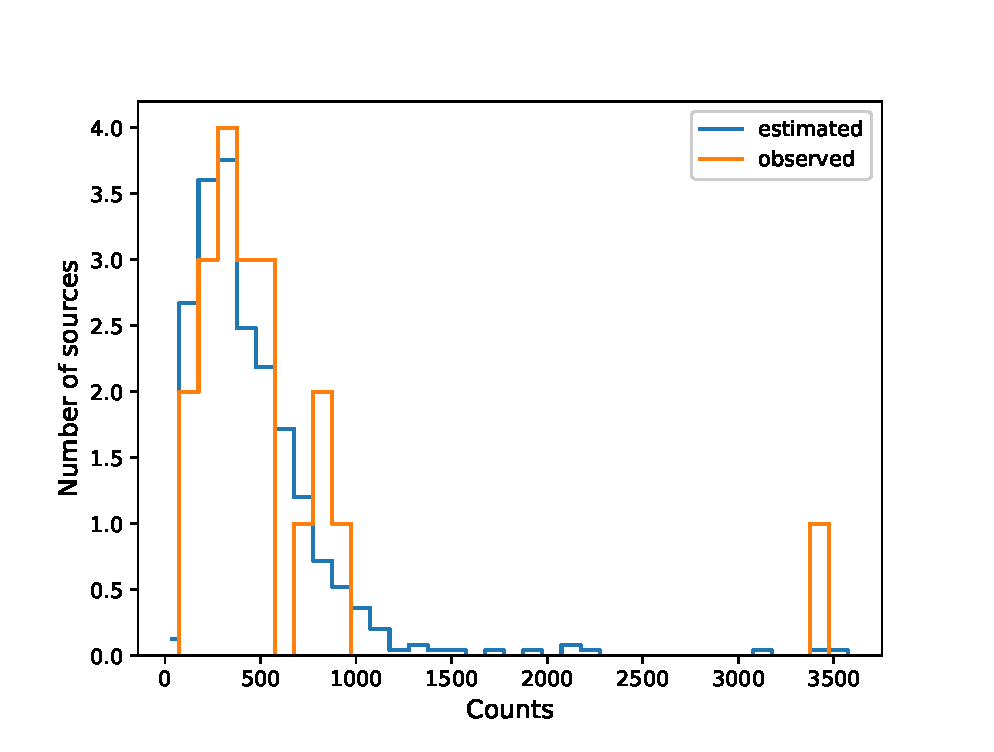
\includegraphics[scale=0.53]{./figure/sim_LW/est_obs.eps}
\caption{The comparison between estimated and the real detected number of sources. \label{fig:NP_sim}}
\end{figure}

\subsection{The estimation for X-ray source population}
Firstly, we assumed that the fraction of polars in the total sample of 847 sources is $\alpha$. The sinusoidal variation happens in "two-pole" situation, which takes $90^\circ$ in total $360^\circ$. Then we can set 25\% as the upper limit for polars with sinusoidal variation intrinsically. We assumed the even distribution for amplitude from 0.5 to 0.9 and took the simulation results for P=5540s and P=45540s as the detection rate for period under(60\% of the total number) and beyond the period gap(40\% of the total number). The value of 60\% and 40\% are estimated from Figure \ref{fig:N_P}. Then we set width=100 for our binning of counts, from 75 to 3575, which consist nearly all detected sources. The predicted number of periodic sources which "should" be detected in each bin is calculated by:
\begin{equation}
Np_{i}=N_i\times DR \times 25\% \times 847 \times \alpha	
\end{equation}
$N_i$ is the product of number of sources detected in the bin. DR denotes the detection rate weighted from simulation. Then we sum all $Np_{i}$ together and force it equals to 20,  getting $\alpha$ about 16\%. The comparison between $Np_{i}$ and the real detected 20 periodic sources(two determined IPs excluded) are plotted in Figure \ref{fig:NP_sim}. The perfect agreement between their population proves the validity of estimation.

Since the real luminosity function should be gentle than that of  total sample, which means there could be more polars at the bright band, then it demanding lower numbers of polar to balance the high detection rate for bright sources. 
In general, the 16\% should be treated as the upper limit for polars, especially when we considered all the 20 sources(already excluding the two IPs) are polars. 

While for DNe, we are constrained by lack of reliable X-ray luminosity function(XLF). We have already set the three as the upper limit of DNe. The steeper XLF for DNe than the XLF for total sample would only contribute the lower limit for their proportion. This conflict increases the  uncertainty of estimation. Here we still present the estimation for fraction of DNe.
Intrinsically, the eclipse of white dwarf depends on the inclination angle, radius of companion star and orbit. If we set $\beta$ as probability of eclipsing, $i$ as inclination, $R_1$,$R_2$,$R_{orb}$ as radius of WD, companion star and orbit respectively. Then the $\beta$ need to fullfill:
\begin{equation}
{R_{orb}\times cos(90-\beta)}\leq { R_1+R_2}
\end{equation}
We took parameters from simulation operated by \citep{2011ApJS..194...28K}, in which $R_1$ is fixed at when $M_{WD}$ equals 0.75 solar mass. Assuming that inclination is even distributed in $(0,90^\circ)$, the probability of eclipsing(hereafter EP) are plotted in Figure \ref{fig:simpCV}.

\begin{figure}[ht!]
\centering
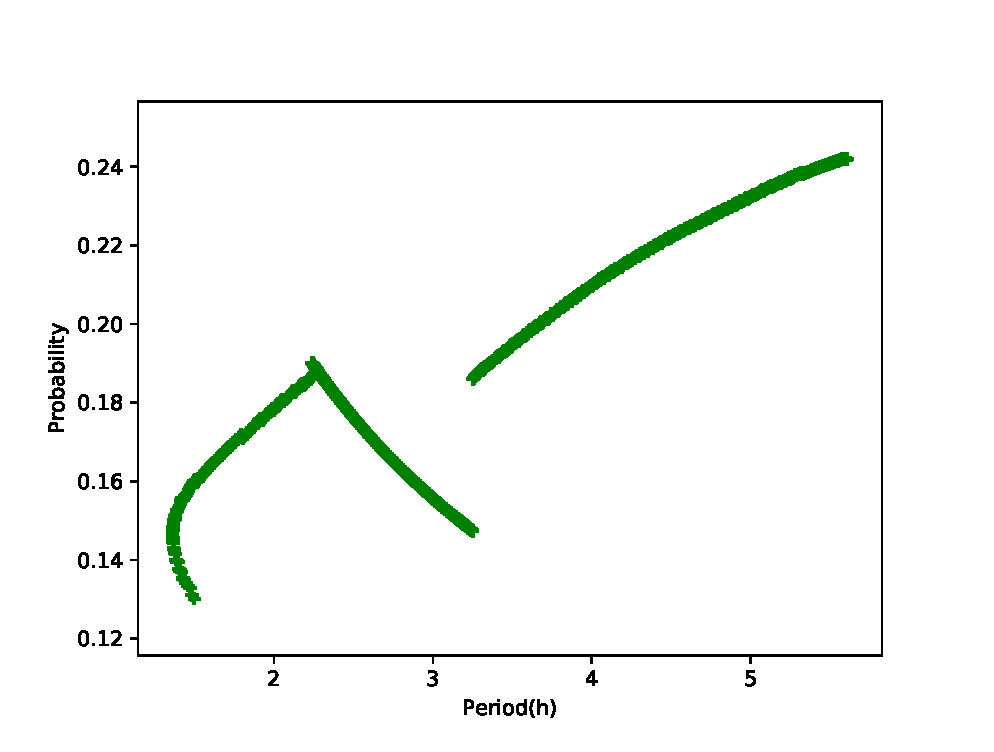
\includegraphics[scale=0.55]{./figure/p_inCV.eps}
\caption{Probability of eclipsing in CVs. The break around 3.2hours resulted by different model for CVs beyond and below the period gap.\label{fig:simpCV}}
\end{figure}
We utilized the simulation results of 5258s and 15258s as the detection rate for period under(75\% of the total number) and beyond the period gap(25\% of the total number). The fraction was taken from the DNe distribution in solar neighborhood. Besides, EP was chosen as 0.18 and 0.20 for this two types.
Similarly, the predicted number of periodic non-mCVs which "should" be detected in each counts bin is:
\begin{equation}
Np_{i}=N_i\times DR \times EP \times 847 \times \alpha	
\end{equation}
Since the sum of $Np_{i}$ was assigned as three, the $\alpha$ would be around 0.67 if we set $\rm 10^{32}~erg~s^{-1}$ (roughly corresponding 675 counts) as the upper limit of luminosity for DNe. The rationality of the limit has been proved by the DNe sample from solar neighborhood in \citep{2016ApJ...818..136X}, based on Suzaku observation. The uncertainty of this fraction comes from our limited acquaintance about XLF for DNe, and the subjective diagnostic for the phase-folded light curve. 
\section{Summary}\label{sec:summary}

1. We have discovered 22 periodic sources with 24 signal in the LW by using GL method, including 10 of them already found by LS method in \cite{2012ApJ...746..165H}. Their luminosity range locates at $\rm 10^{31}-10^{33}~erg~s^{-1} $.The general feature of these 22 sources resembles that of polars. Three of them with narrow dip are likely DNe. Two of them are determined as IP.

2.  We estimate the mass of WD from two sources with great identification for Fe XXVI and Fe XXV emission lines, i.e. 0.8 $M_\odot$ for \#21(\#22), and 0.5(1.0) $M_\odot$ for \#23 if being an IP(DN). 

3. We provide well-constrained fraction of polars in the whole sample, i.e, 16\% as the upper limit. The estimation on fraction of non-mCVs is about 67\% while the certainty is restricted by limited appreciation about their XLF. Combined with the period distribution, we conclude that the periodic sources are mainly polars with relatively harder spectra, especially in the luminosity range that lower than $\rm 10^{32}~erg~s^{-1}$. Besides, the H sources (L>$\rm 10^{32}~erg~s^{-1}$), whose emission is mostly contributed by IPs, indicate  $M_{WD} \sim 0.8 M_\odot$, consistent with the previous result $0.8\pm 0.07 M_\odot$ in \citep{2018ApJ...853..182Y}.

4. The lower luminosity and narrow eclipsing model for orbital modulation reduced the detection rate simultaneously for periodicity. That may explain why we had no trace on non-mCVs in GCR in earlier period searching work.

5. We proved the higher detection rate, more usage of data and ignorance of observation gap for GL method compared with LS method. It is noteworthy that the shape of light curve in GL method could be modified according to different scenarios. It was applied on detection of planetary transits by using customized eclipsing model \citep{2002A&A...395..625A}. For the utility of GL method, there is still room for improvement in the future.


\begin{deluxetable*}{LCCCCCCR}
%\tablenum{1}
\tablecaption{X-ray spectral properties of the periodic sources \label{tab:spec}}
\tablewidth{0pt}
\tablehead{
\colhead{ID} & \colhead{$N_{H}$} & \colhead{$T_b$} &
\colhead{$I_{6.4}/I_{6.7}$} & \colhead{$I_{7.0}/I_{6.7}$} & \colhead{$I_{6.7}$}& \colhead{$\chi^2/dof$} &  \colhead{Luminosity(1-8keV)} 
\\
\colhead{} & \colhead{$10^{22} cm^{-2}$} & \colhead{keV} & 
\colhead{} & \colhead{} & \colhead{$\rm 10^{-8} ph~ cm^{-2}~s^{-1} $}&\colhead{}  & \colhead{$\rm 10^{31} ~erg~s^{-1}$}
}
\decimals
\decimalcolnumbers
\startdata
1^\dag & $0.51^{+0.75}_{-0.34}$ & 40(fixed) &-&-&-& 1.14/5  & $1.82^{+0.64}_{-0.51}$
\\
2 & $2.17^{+0.54}_{-0.46}$ & $20.66^{+56.89}_{-9.92}$ &-&-&-& 0.86/78  & $23.11^{+2.70}_{-2.01}$
\\
3 & $1.34^{+0.70}_{-0.40}$ & $46.41^{+46.05}_{-38.52}$ &-&-&-& 0.98/33  & $6.61^{+1.05}_{-0.77}$
\\
4 & $1.15^{+0.69}_{-0.50}$ & $11.26^{+53.31}_{-4.71}$ &-&-&-& 0.91/27  & $22.50^{+2.94}_{-4.42}$
\\
5 & $1.02^{+0.27}_{-0.23}$ & 40(fixed) &-&-&-& 1.00/33 &  $5.59^{+0.77}_{-0.70}$
\\
6 & $1.82^{+0.57}_{-0.50}$ & $6.90^{+12.38}_{-2.90}$ 
	&-&-&-& 1.12/42 &  $9.23^{+1.24}_{-1.11}$
\\
7 & $1.62^{+0.62}_{-0.49}$ & $41.57^{+42.96}_{-32.34}$ &-&-&-& 0.86/39 &  $6.70^{+0.89}_{-0.81}$
\\
8 & $2.06^{+1.51}_{-0.94}$ & 40(fixed) &-&-&-& 0.93/7 &  $1.76^{+0.54}_{-0.42}$
\\
9 & $1.29^{+1.34}_{-0.67}$ & $20.79^{+95.79}_{-20.79}$ &-&-&-& 1.10/7 &  $3.50^{+1.22}_{-0.86}$
\\
10 & $2.50^{+7.25}_{-1.56}$ & 40(fixed) &-&-&-& 0.85/5 &  $2.14^{+1.76}_{-0.75}$
\\
11 & $1.85^{+0.39}_{-0.33}$ & 40(fixed) &-&-&-& 1.22/47 &  $9.49^{+1.11}_{-1.02}$
\\
12 & $6.23^{+9.67}_{-3.66}$ & 40(fixed) &-&-&-& 0.78/6 &  $7.58^{+5.76}_{-2.93}$
\\
13 & $0.90^{+0.30}_{-0.24}$ & 40(fixed) &-&-&-& 1.15/38 &  $8.48^{+1.12}_{-1.04}$
\\
14^\dag & $0.51^{+0.75}_{-0.34}$ & 40(fixed) &-&-&-&  1.14/5 &  $1.82^{+0.64}_{-0.51}$
\\
15 & $1.46^{+0.48}_{-0.38}$ & 40(fixed) &-&-&-&  1.16/42 & $12.85^{+1.77}_{-1.61}$
\\
16 & $0.89^{+0.18}_{-0.16}$ & 40(fixed) &-&-&-&  1.43/51  & $8.47^{+0.88}_{-0.83}$
\\
17 & $2.68^{+0.63}_{-0.52}$ & 40(fixed) &-&-&-&  0.75/36 & $11.28^{+1.61}_{-1.45}$
\\
18 & $2.01^{+0.92}_{-0.66}$ & 40(fixed) &-&-&-&  0.53/14  & $4.21^{+0.89}_{-0.77}$
\\
19 & $1.82^{+0.10}_{-0.10}$ & 40(fixed) &-&-&-& 0.95/185  & $83.87^{+3.25}_{-3.16}$
\\
20 & $2.09^{+2.45}_{-1.16}$ & $4.04^{+28.24}_{-2.54}$ &-&-&-& 1.04/12  & $5.39^{+1.81}_{-1.47}$
\\
21^\ddag & $2.83^{+0.25}_{-0.23}$ & 40(fixed) & $0.47^{+0.35}_{-0.24}$ & $0.91^{+0.38}_{-0.60}$ & 31.71 & 1.10/147  & $59.99^{+3.25}_{-3.12}$
\\
22^\ddag & $2.83^{+0.25}_{-0.23}$ & 40(fixed) & $0.47^{+0.35}_{-0.24}$ & $0.91^{+0.38}_{-0.60}$ &  31.71 & 1.10/147  & $59.99^{+3.25}_{-3.12}$
\\
23 & $1.83^{+0.44}_{-0.37}$ & 40(fixed) & $ <0.52 $& $0.51^{+0.80}_{-0.47}$ & 10.09 & 1.47/35  & $9.23^{+1.22}_{-1.13}$
\\
24 & $0.83^{+0.83}_{-3.31}$ & $2.30^{+1.59}_{-0.85}$ &-&-&-&  0.80/2 & $0.77^{+7.82}_{-0.36}$
\enddata
\tablecomments{Columns:\\
(1) Source sequence number assigned in the order of increasing period. The same source with multiple period signal was denoted as \dag and \ddag.\\
 (2) An estimate of the absorption coefficient from spectral model fits.\\
 (3) The best-fit plasma temperature if constrained well. Otherwise we fix it at 40 keV.\\
 (4) or (5) Flux ratios of the 6.4 or 7.0 keV line to the 6.7 keV line.\\
 (6) The intensity of 6.7 keV line.\\
 (7)The Reduced $\chi^2$ and degrees of freedom (dof) of best-fit.\\
 (8) The estimate of luminosity for source distance at 8 kpc.}
\end{deluxetable*}

\begin{figure*}[htbp]
\centering
\rotatebox[origin=c,x=11pt,y=146pt]{270}{\includegraphics[width = 0.7\textwidth]{./figure/LW/pCV_brem.eps}}
\caption{Cumulative spectra with the best-fit model($phabs\times (bremsstrahlung+gaussian+gaussian+gaussian) $).
The spectrum for H, L set of periodic sources are plotted in red and black respectively. \label{fig:pCV_spec}}
\end{figure*}

\begin{deluxetable*}{CCCCCCC}
%\tablenum{1}
\tablewidth{25cm}
\tablecaption{Spectral fit results for the periodic sources (combined) \label{tab:pCV_spec}}
\tablehead{
\colhead{Set} & \colhead{$N_{H_{phabs}}$} & \colhead{$T_{b}$}&
\colhead{$I_{6.4}/I_{6.7}$} & \colhead{$I_{7.0}/I_{6.7}$} & \colhead{$I_{6.7}$}& \colhead{$\chi^2/dof$}
\\
\colhead{} & \colhead{$10^{22} cm^{-2}$} & \colhead{keV} & 
\colhead{} & \colhead{} & \colhead{$\rm 10^{-8} ph~ cm^{-2}~s^{-1} $}&\colhead{}
}

\decimals
\decimalcolnumbers
\startdata
H & $1.99^{+0.10}_{-0.97}$ & 40(fixed) &  $0.28^{+0.06}_{-0.05}$ & $0.78^{+0.10}_{-0.09}$  & $8.76^{+3.57}_{-3.57}$ & 1.19/205
\\
L & $1.33^{+0.12}_{-0.11}$ & 40(fixed) & $0.03^{+0.08}_{-0.03}$  & $0.14^{+0.15}_{-0.14}$ & $2.53^{+1.10}_{-1.10}$ & 1.09/168
\enddata
\end{deluxetable*}

\clearpage
\newpage

\appendix
\section{A brief introduction about GL method}\label{GL}
The basic rules for Bayesian probabilities are the sum rule:
\begin{equation}
p(H_i|I)+p(\bar{H_i}|I)	=1
\end{equation}
\indent
And the product rule:
\begin{equation}\label{2.2}
p(H_i,D|I)=p(H_i|I)\cdot p(D|H_i,I)=p(D|I)\cdot p(H_i|D,I)
\end{equation}
\indent
From equation \ref{2.2} we could easily derive Bayes's theorem.
\begin{equation}\label{2.5} 
p(H_i|D,I)=p(H_i|I)\cdot {p(D|H_i,I)\over p(D|I)}
\end{equation}
\indent
The symbols in this work follow the same expression used in \citep{1992ApJ...398..146G}. Throughout this work, these symbols could be briefly practically understood. $H_i$ signifies model, $D$ signifies dataset, $I$ represents the ensemble of all the hypotheses considered i.e. all the model used.

 GL method employs stepwise function for periodic signal. Each model has $(m+2)$ parameters: angular frequency $\omega={2\pi/P}$, P represents period; phase parameter $\phi$; and m values $r_j$, signifies the counts rate in each phase bin where j=1 to m. The following we replace $H_i$ with $M_i$ to denote the model where i represents the number of bins in stepwise model. Then the Bayes's theorem can be written as:
 \begin{equation}\label{2.11}
 p(M_i|D,I)=p(M_i|I)\cdot {p(D|M_i,I)\over p(D|I)}
 \end{equation}
 
We could write $I=M_1+M_2+M_3+\cdots$, where ``+'' stands for ``or''. Thus the proposition ($M_i$,I) is true if and only if model $M_i$ is true i.e. ($M_i$,I) = $M_i$. GL method defines odds ratio to make the model comparison.
\begin{equation}\label{2.12}
O_{ij}={p(M_i|D,I)\over p(M_j|D,I)}={p(M_i|I)\over p(M_j|I)}\cdot {p(D|M_i)\over p(D|M_j)}
\end{equation}

Note that $M_1$ means constant model, $M_i$(i=2,3,4 $\cdots N_{mod}$, where $N_{mod}$ is the total number of models considered.) represents periodic model. The probabilities for each model can be deduced by \ref{2.12}
\begin{equation}\label{6}
p(M_i|D,I)=O_{i1}\cdot p(M_1|D,I)
\end{equation}
\begin{equation}\label{7}
p(M_1|D,I)={{\sum_{j=1}^{N_{mod}} p(M_j|D,I)}\over {\sum_{j=1}^{N_{mod}} O_{j1}}}
={1\over {\sum_{j=1}^{N_{mod}} O_{j1}}}	
\end{equation}

Substitute \ref{7} into \ref{6}, we got
\begin{equation}\label{2.13}
p(M_i|D,I)={O_{i1}\over {\sum_{j=1}^{N_{mod}} O_{j1}}}
\end{equation}

Then the probability that the signal is periodic is :
\begin{equation}\label{5.2}
p(M_m(m>1)|D,I)={{\sum_{m=2}^{m_{max}} O_{m1}}\over {1+\sum_{m=2}^{m_{max}} O_{m1}}}
\end{equation}

The odds ratio can be calculated by the probability for model:
\begin{equation}
O_{m1}={{p(M_m|D.I)}\over {p(M_1|D.I)}}
\end{equation}

Using Bayes's theorem shown as \ref{2.11},
\begin{equation}\label{11}
O_{m1}={{p(M_m|I)\cdot p(D|M_m)}\over {p(M_1|I)\cdot p(D|M_1)}}
\end{equation}

Following the same assignment by \citep{1992ApJ...398..146G}, we also consider the probability of periodic and aperiodic signals are the same. Then the priors for model can be written explicitly as :
\begin{equation}\label{12}
p(M_1|I)={1\over 2}	
\end{equation}
\begin{equation}\label{13}
p(M_m|I)={1\over {2\nu}}	, \quad \nu =m_{max}-1
\end{equation}

Since the essence of the algorithm is not our subject, we directly introduce the equation 5.27 in GL method as follows. It must be emphasized that this equation worked for the situation when the period and phase are both unknown. 
\begin{equation}\label{5.27}
p(D|M_m)={{{\Delta t}^N (m-1)! N! \gamma(N+1,A_{max})T}\over{2\pi A_{max} (N+m-1)!T^{N+1} \ln(\omega_{hi}/\omega_{lo})}}\times {\int_{w_{lo}}^{w_{hi}}}{{d\omega}\over{\omega}}\times {\int_0^{2\pi}d\phi{m^N\over W_m(\omega,\phi)}}	
\end{equation}

Substituting $m=1$ into \ref{5.27}, we got:
\begin{equation}\label{15}
p(D|M_1)={{{\Delta t}^N N!\gamma(N+1,A_{max})T}\over {A_{max}N!T^{N+1}}}
\end{equation}

Substituting \ref{12}, \ref{13}, \ref{5.27}, \ref{15} into \ref{11}, the odds ratio could be written as follows, which is the same as equation 5.28 in GL method:
\begin{equation}\label{16}
O_{m1}={1\over{2\pi \nu \ln(\omega_{hi}/\omega_{lo})}} {{N+m-1}	\choose N}^{-1}\times {\int_{w_{lo}}^{w_{hi}}}{{d\omega}\over{\omega}}\times {\int_0^{2\pi}d\phi{m^N\over W_m(\omega,\phi)}} 
\end{equation}

In astronomical dataset, the observation always brings data gaps. For example, when the period is long and the exposure time for single observation is low, different bins may not be covered fairly. Then the initial assumptions above mentioned may fail, leading to some fake detections especially at low frequencies. In appendix B to \citep{1992ApJ...398..146G}, a solution to this problem has been proposed. They defined a weighting factor $S(\omega,\phi)$, where ${\tau_{j}(\omega,\phi)}$ signifies the exposure time in each bin:
\begin{equation}\label{A17}
S(\omega,\phi)={\prod_{j=1}^m s_j^{-n_j}}
\end{equation}
\begin{equation}
s_j(\omega,\phi)={{\tau_{j}(\omega,\phi)}\over {T/m}}
\end{equation}
\indent
Then the odds ratio should be modified as:
\begin{equation}\label{19}
O_{m1}={1\over{2\pi \nu \ln(\omega_{hi}/\omega_{lo})}} {{N+m-1}	\choose N}^{-1}\times {\int_{w_{lo}}^{w_{hi}}}{{d\omega}\over{\omega}}\times {\int_0^{2\pi}d\phi{S(\omega,\phi)m^N\over W_m(\omega,\phi)}} 
\end{equation}

Ultimately, the probability of whether the dataset is periodic is:
\begin{equation}\label{20}
p(periodic)={{\sum_{m=2}^{m_{max}} O_{m1}}\over {1+\sum_{m=2}^{m_{max}} O_{m1}}}
\end{equation}

The posterior probability of the frequency indicates the period of the signal:
\begin{equation}\label{19}
O_{m1}(\omega)={1\over{2\pi \nu}} {{N+m-1}	\choose N}^{-1} \times {\int_0^{2\pi}d\phi{S(\omega,\phi)m^N\over W_m(\omega,\phi)}} 
\end{equation}

The period locates at $P=2\pi /\omega $ when $O_{m1}(\omega)$ takes the highest value.

\section{Figures for periodic CVs }
\begin{figure*}[htbp]
    \centering
    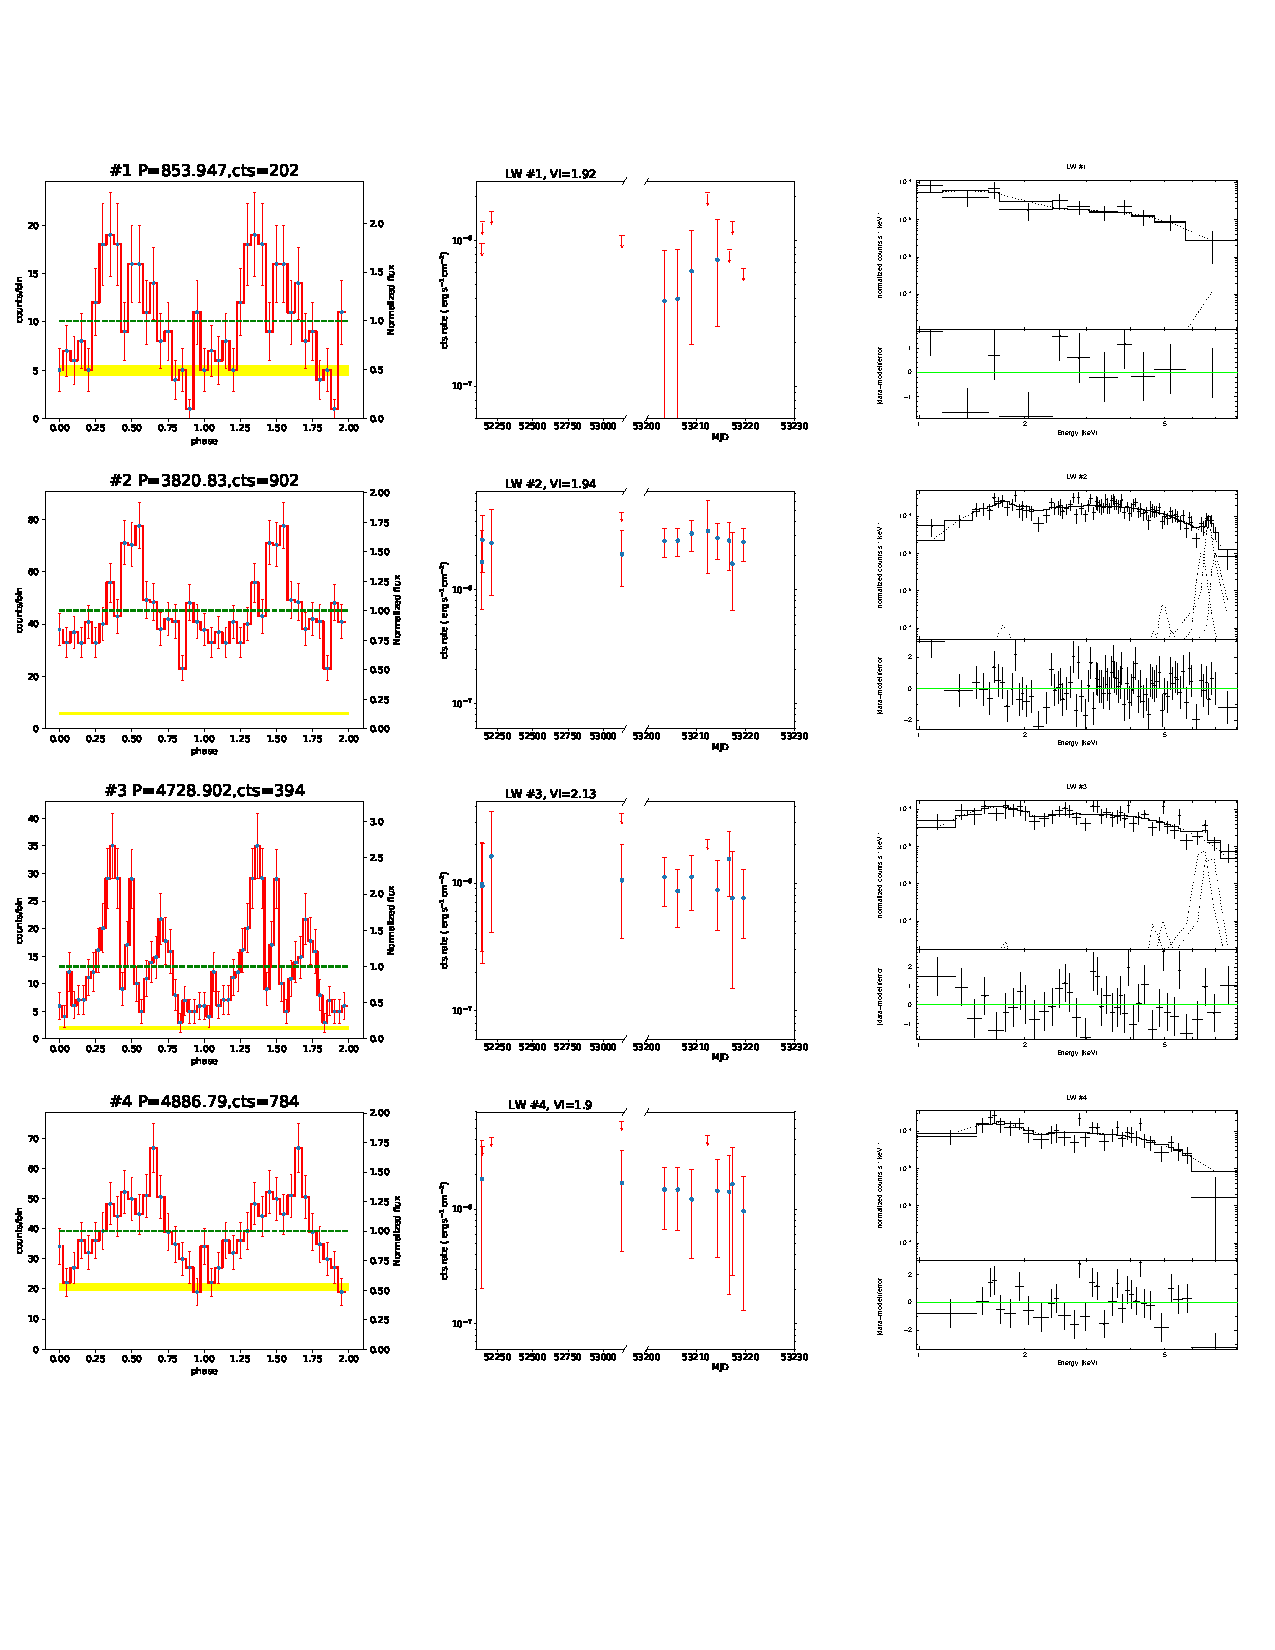
\includegraphics[page=1,scale=0.90,trim=5 50 0 20,clip]{plot_figure_LW.pdf}
    \caption{First figure \label{fig:Figure_p}}
  \end{figure*}
  
  \begin{figure*}[ht]
    \ContinuedFloat
    \captionsetup{list=off,format=cont}
    \centering
    \includegraphics[page=2,scale=0.90,trim=5 50 0 20,clip]{plot_figure_LW.pdf}
    \caption{First figure continued}
  \end{figure*}

  \begin{figure*}[ht]
  \ContinuedFloat
  \captionsetup{list=off,format=cont}
    \centering
    \includegraphics[page=3,scale=0.90,trim=5 50 0 20,clip]{plot_figure_LW.pdf}
    \caption{First figure continued}
  \end{figure*}
  
   \begin{figure*}[ht]
  \ContinuedFloat
  \captionsetup{list=off,format=cont}
    \centering
    \includegraphics[page=4,scale=0.90,trim=5 50 0 20,clip]{plot_figure_LW.pdf}
    \caption{First figure continued}
  \end{figure*}
  
  \begin{figure*}[ht]
  \ContinuedFloat
  \captionsetup{list=off,format=cont}
    \centering
    \includegraphics[page=5,scale=0.90,trim=5 50 0 20,clip]{plot_figure_LW.pdf}
    \caption{First figure continued}
  \end{figure*}
  
  \begin{figure*}[ht]
  \ContinuedFloat
  \captionsetup{list=off,format=cont}
    \centering
    \includegraphics[page=6,scale=0.90,trim=5 50 0 20,clip]{plot_figure_LW.pdf}
    \caption{First figure continued}
  \end{figure*}


\clearpage
\newpage
%% For this sample we use BibTeX plus aasjournals.bst to generate the
%% the bibliography. The sample63.bib file was populated from ADS. To
%% get the citations to show in the compiled file do the following:
%%
%% pdflatex sample63.tex
%% bibtext sample63
%% pdflatex sample63.tex
%% pdflatex sample63.tex

\bibliography{sample63}{}
\bibliographystyle{aasjournal}


\end{document}

% End of file `sample63.tex'.
